\documentclass[11pt]{article}
\usepackage[margin=1.1in]{geometry}
\usepackage{amsmath,amssymb,amsthm}
\usepackage{graphicx}
\usepackage[hidelinks]{hyperref}
\usepackage{microtype}

\newtheorem{lemma}{Lemma}
\newtheorem{proposition}{Proposition}

\newcommand{\Tr}{\operatorname{Tr}}
\newcommand{\Var}{\operatorname{Var}}
\newcommand{\rms}{\operatorname{rms}}
\newcommand{\ad}{\operatorname{ad}}

\title{Exact disorder statistics of adjoint observables in the SYK model,\\
with applications to the DSSYK$_\infty$\,--\,'t~Hooft correspondence}

% TODO(author): confirm author line and affiliation before circulating.
\author{Henry Donahue}
\date{July 2026 --- draft, not for distribution}

\begin{document}
\maketitle

\begin{abstract}
Miyashita, Sekino and Susskind have argued that individual disorder realizations
of the double-scaled SYK model at infinite temperature enjoy an emergent
$O(N)$ (or $U(N)$) symmetry, because singlet observables self-average with
variance $\sim p!/N^p$ and symmetry-violating (adjoint) observables are bounded
by $e^{-a\sqrt N}$ for every $a$ [arXiv:2607.05678, Eqs.~(3.27)--(3.28)]. The
supporting counting was given through two example diagrams, and, as far as we
are aware, no systematic derivation has appeared. We supply one for the
quantities that control the claim. For the adjoint bilinear
$B_{jk}=\Tr(\psi_j H\psi_k H)/\dim$ we prove the closed forms
$\Var(B_{jk})=4\sigma^4\binom{N-2}{p-1}$ ($j\neq k$) and
$\mathbb E[B_{jj}]=\sigma^2\binom{N}{p}\,(1-2p/N)$, with
$\sigma^2=p!/N^{p-1}$, exact at every $(N,p)$; the singlet second moment has
relative variance exactly $2/\binom{N}{p}$. These confirm the published
leading-order counting and sharpen it: along the double-scaling line
$p=\sqrt{\lambda N}$ the typical symmetry violation obeys
$\ln\rms(B_{jk})=-\tfrac14\sqrt{\lambda N}\,\ln N\,(1+o(1))$, beating
$e^{-a\sqrt N}$ for every $a$, while at fixed $p$ --- the regime where the
proposed 't~Hooft comparison must be performed --- the suppression is only the
power law $N^{-(p-1)/2}$. The vanishing of $\mathbb E[B_{jj}]$ at $p=N/2$
explains an artifact visible in exact-diagonalization studies. We verify the
formulas three independent ways. As a byproduct of setting up the $U(N)$
(Dirac) sector we record several corrections to the operator dictionary of the
singlet tower $M_n=\psi_i^\dagger(d^n\!/dt^n)\psi_i$: $M_1=-(p/2)\,iH$ (not
$H$), $M_2=-\sum_i\dot\psi_i^\dagger\dot\psi_i$ (opposite sign to the published
identity), $M_n^\dagger=(-1)^nM_n$ only for $n\le2$, the relevant CP operation
is necessarily the \emph{unitary} particle--hole map, and for $n\ge2$ the raw
$M_n$ carry both CP channels, so the assignment $\mathrm{CP}=(-1)^{n+1}$ is a
statement about CP-resolved correlators.
\end{abstract}

\section{Introduction}

The double-scaled SYK model at infinite temperature (DSSYK$_\infty$) has been
proposed as a holographic description of the static patch of de~Sitter space,
and, in the flat-space limit, as dual to the 't~Hooft model of large-$N$
two-dimensional QCD \cite{MSS2607,SS2501,MSS2506}. A load-bearing step in that
program is the claim that a \emph{single} disorder realization behaves, in the
double-scaled limit, as if it were $O(N)$ (Majorana) or $U(N)$ (Dirac)
invariant: singlet observables self-average,
\begin{equation}
\Var\langle W\rangle \;\sim\; \frac{p!}{N^p},
\tag{3.27 of \cite{MSS2607}}
\end{equation}
and symmetry-violating observables are smaller than $e^{-a\sqrt N}$ for every
$a$ (their Eq.~3.28). In \cite{MSS2607} this is supported by comparing two
diagrams; the diagrammatic rules are developed in \cite{SS2501}, but that paper
concerns the ensemble-averaged $1/N$ expansion --- the variance application, and
in particular its prefactors, appear not to have been published anywhere.

This note closes that gap for the observables that control the claim, using
nothing beyond Wick's theorem and Majorana trace combinatorics, and draws two
consequences relevant to any quantitative test of the proposed duality. All
formulas here are implemented and machine-verified in an accompanying
repository.\footnote{\texttt{syk-self-averaging/exact\_wick.py} and
\texttt{dirac.py}; every displayed equation is asserted by the test suite,
including a literal enumeration of all Wick contractions at small $(N,p)$.}

\section{Setup}

We use the conventions of \cite{MSS2607}. $N$ Majorana fermions
$\{\psi_a,\psi_b\}=2\delta_{ab}$, Hamiltonian
\begin{equation}
H=i^{p/2}\!\!\sum_{i_1<\cdots<i_p}\!\! J_{i_1\cdots i_p}\,
\psi_{i_1}\cdots\psi_{i_p}
\;\equiv\;\sum_c J_c\,\Gamma_c ,
\qquad
\Gamma_c=i^{p/2}\psi_{c_1}\cdots\psi_{c_p},
\end{equation}
with $c$ ranging over ascending $p$-subsets, $p$ even, and independent Gaussian
couplings of variance
\begin{equation}
\sigma^2 \;\equiv\; \Var(J_c) \;=\; \frac{p!}{N^{p-1}} .
\end{equation}
Infinite-temperature expectation values are normalized traces,
$\langle X\rangle=\Tr X/\dim$. Two standard facts we use repeatedly:
$\Gamma_c^2=1$, and the normalized trace of a product of Majoranas vanishes
unless every index appears an even number of times.

\section{The singlet rate}

The simplest singlet is the second moment
$m_2=\langle H^2\rangle=\sum_c J_c^2$: a sum of $\binom{N}{p}$ i.i.d.\
squared Gaussians, so
\begin{equation}
\frac{\Var(m_2)}{(\mathbb E\,m_2)^2}=\frac{2}{\binom{N}{p}}
=\frac{2\,p!}{N^p}\prod_{k=1}^{p-1}\Bigl(1-\frac kN\Bigr)^{-1}.
\label{eq:singlet}
\end{equation}
This is the paper's $p!/N^p$ with its exact prefactor: a factor $2$ (the Wick
multiplicity) and a factor $\prod(1-k/N)^{-1}\approx e^{+p^2/2N}$ which is
$O(1/N)$ at fixed $p$ but order one on the double-scaling line
$\lambda=p^2/N$ fixed. Exact diagonalization confirms
Eq.~\eqref{eq:singlet} at $N\le18$, and confirms that the higher moments
$m_4,m_6$ self-average at the same combinatorial $1/\binom{N}{p}$ rate.
(We stress the logical status: Eq.~\eqref{eq:singlet} is an elementary identity
that holds independently of any diagrammatic argument; the nontrivial content
of the self-averaging claim lies in the adjoint sector, to which we now turn.)

\section{Exact statistics of the adjoint bilinear}

The natural symmetry-violation observable --- the one measured in
exact-diagonalization studies --- is the $H$-dressed adjoint bilinear
\begin{equation}
B_{jk}\;=\;\bigl\langle \psi_j\,H\,\psi_k\,H\bigr\rangle
\;=\;\sum_{c,d}J_cJ_d\,T_{cd},
\qquad
T_{cd}\;=\;\bigl\langle\psi_j\Gamma_c\psi_k\Gamma_d\bigr\rangle .
\end{equation}
In the $O(N)$-invariant ensemble $\mathbb E[B_{jk}]\propto\delta_{jk}$, so for
$j\neq k$ a nonzero $B_{jk}$ is a finite-$N$, single-instance symmetry
violation.

\begin{lemma}[trace selection]\label{lem:selection}
For $j\neq k$, $T_{cd}\neq0$ if and only if the symmetric difference
$c\,\triangle\,d=\{j,k\}$, i.e.
\begin{equation}
d=(c\setminus\{j\})\cup\{k\}\quad(j\in c,\ k\notin c)
\qquad\text{or}\qquad j\leftrightarrow k .
\end{equation}
\end{lemma}

\begin{proof}
The trace vanishes unless every index of
$\psi_j\Gamma_c\psi_k\Gamma_d$ appears an even number of times. Elements of
$c\cap d$ appear twice; elements of $c\,\triangle\,d$ once; $j$ and $k$
contribute one each. Evenness forces $c\,\triangle\,d=\{j,k\}$, and $|c|=|d|$
selects the two stated cases.
\end{proof}

\begin{lemma}[trace values]\label{lem:values}
Write $c=e\cup\{j\}$, $d=e\cup\{k\}$ with $|e|=p-1$, $j,k\notin e$. Then
\begin{equation}
T_{cd}\;=\;T_{dc}\;=\;i^{\,p}\,\sigma_c\,\sigma_d\,(-1)^{(p-1)(p-2)/2},
\qquad \sigma_c,\sigma_d\in\{\pm1\},
\end{equation}
so that $T_{cd}^2=T_{cd}T_{dc}=+1$ for every admissible pair. On the diagonal,
$\langle\psi_j\Gamma_c\psi_j\Gamma_c\rangle=-1$ if $j\in c$ and $+1$
otherwise.
\end{lemma}

\begin{proof}
Pull the distinguished Majorana to the front of the ascending product:
$\Gamma_c=i^{p/2}\sigma_c\,\psi_j\Psi_e$ with
$\sigma_c=(-1)^{\#\{a\in e\,:\,a<j\}}$ and $\Psi_e$ the ascending product over
$e$; likewise $\Gamma_d=i^{p/2}\sigma_d\,\psi_k\Psi_e$. Then, using
$\psi^2=1$ and $\Psi_e\psi_k=(-1)^{p-1}\psi_k\Psi_e$,
\begin{equation}
\psi_j\Gamma_c\psi_k\Gamma_d
= i^{\,p}\sigma_c\sigma_d\,(\psi_j\psi_j)\,\Psi_e\,(\psi_k\psi_k)\,\Psi_e
= i^{\,p}\sigma_c\sigma_d\,\Psi_e^2
= i^{\,p}\sigma_c\sigma_d\,(-1)^{(p-1)(p-2)/2},
\end{equation}
a $c$-number; the computation for $T_{dc}$ differs by moving each of
$\psi_j,\psi_k$ once through $\Psi_e$, producing two compensating signs
$(-1)^{p-1}$, hence $T_{dc}=T_{cd}$. Squaring, $i^{2p}=(-1)^p=+1$ for even
$p$. For the diagonal statement the same normal-form manipulation gives
$\psi_j\Gamma_c\psi_j\Gamma_c=i^{\,p}(-1)^{(p-1)(p-2)/2}$ for $j\in c$, whose
sign is $-1$ for every even $p$ (the exponent
$p/2+(p-1)(p-2)/2=p^2/2-p+1$ is odd), while for $j\notin c$ one finds
$\Gamma_c^2=+1$.
\end{proof}

\begin{proposition}[exact adjoint statistics]\label{prop:main}
For $j\neq k$,
\begin{equation}
\boxed{\;\mathbb E[B_{jk}]=0,\qquad
\Var(B_{jk})\;=\;4\,\sigma^4\binom{N-2}{p-1},\;}
\label{eq:var}
\end{equation}
and on the diagonal
\begin{equation}
\boxed{\;\mathbb E[B_{jj}]\;=\;\sigma^2\!\left[\binom{N}{p}-2\binom{N-1}{p-1}\right]
=\sigma^2\binom{N}{p}\Bigl(1-\frac{2p}{N}\Bigr).\;}
\label{eq:diag}
\end{equation}
\end{proposition}

\begin{proof}
$\mathbb E[B_{jk}]=\sigma^2\sum_cT_{cc}$ vanishes for $j\neq k$ by
Lemma~\ref{lem:selection}. For the variance, Wick's theorem gives three
pairings of $\mathbb E[J_cJ_dJ_{c'}J_{d'}]$; the $\langle cd\rangle\langle
c'd'\rangle$ pairing vanishes for the same reason, leaving
\begin{equation}
\Var(B_{jk})=\sigma^4\Bigl[\sum_{c,d}T_{cd}^2+\sum_{c,d}T_{cd}T_{dc}\Bigr]
=\sigma^4\bigl[2\binom{N-2}{p-1}+2\binom{N-2}{p-1}\bigr],
\end{equation}
using Lemma~\ref{lem:values} and the count of admissible ordered pairs
($j\in c$, $k\notin c$: $\binom{N-2}{p-1}$ choices of $c$, plus the mirrored
case). Eq.~\eqref{eq:diag} follows from the diagonal trace values:
$\binom{N-1}{p-1}$ subsets contain $j$ (each contributing $-1$) and the
remainder contribute $+1$.
\end{proof}

\paragraph{Verification.} Three independent checks are implemented:
(i)~\emph{literal enumeration}: for $(N,p)\in\{(6,2),(6,4),(8,4),(8,6),(10,4)\}$
every $T_{cd}$ is evaluated as a Pauli-string trace and the double sum
performed explicitly; the ratio to Eq.~\eqref{eq:var} is $1$ to machine
precision, pinning every sign in the lemmas.
(ii)~\emph{exact diagonalization}: disorder ensembles (120--200 realizations,
$N\le18$, $p=4,6$; construction validated against the $N\bmod8$
random-matrix classification of the SYK ensemble \cite{GV}) reproduce
$\rms(B_{jk})$ within their $\sim1\%$ sampling errors (Fig.~\ref{fig:main},
right).
(iii)~\emph{consistency with the published counting}: writing
$\Var(B_{jk})=4\,\frac{p(N-p)}{N(N-1)}\,\sigma^4\binom{N}{p}$ exhibits the
result as the ``diagram B'' magnitude $\sigma^4\binom{N}{p}\approx
p!/N^{p-2}$ of \cite{MSS2607} times the index-pinning factor of the two
external adjoint legs --- confirming the published leading-order counting while
supplying the prefactor it necessarily lacked.

\begin{figure}[t]
\centering
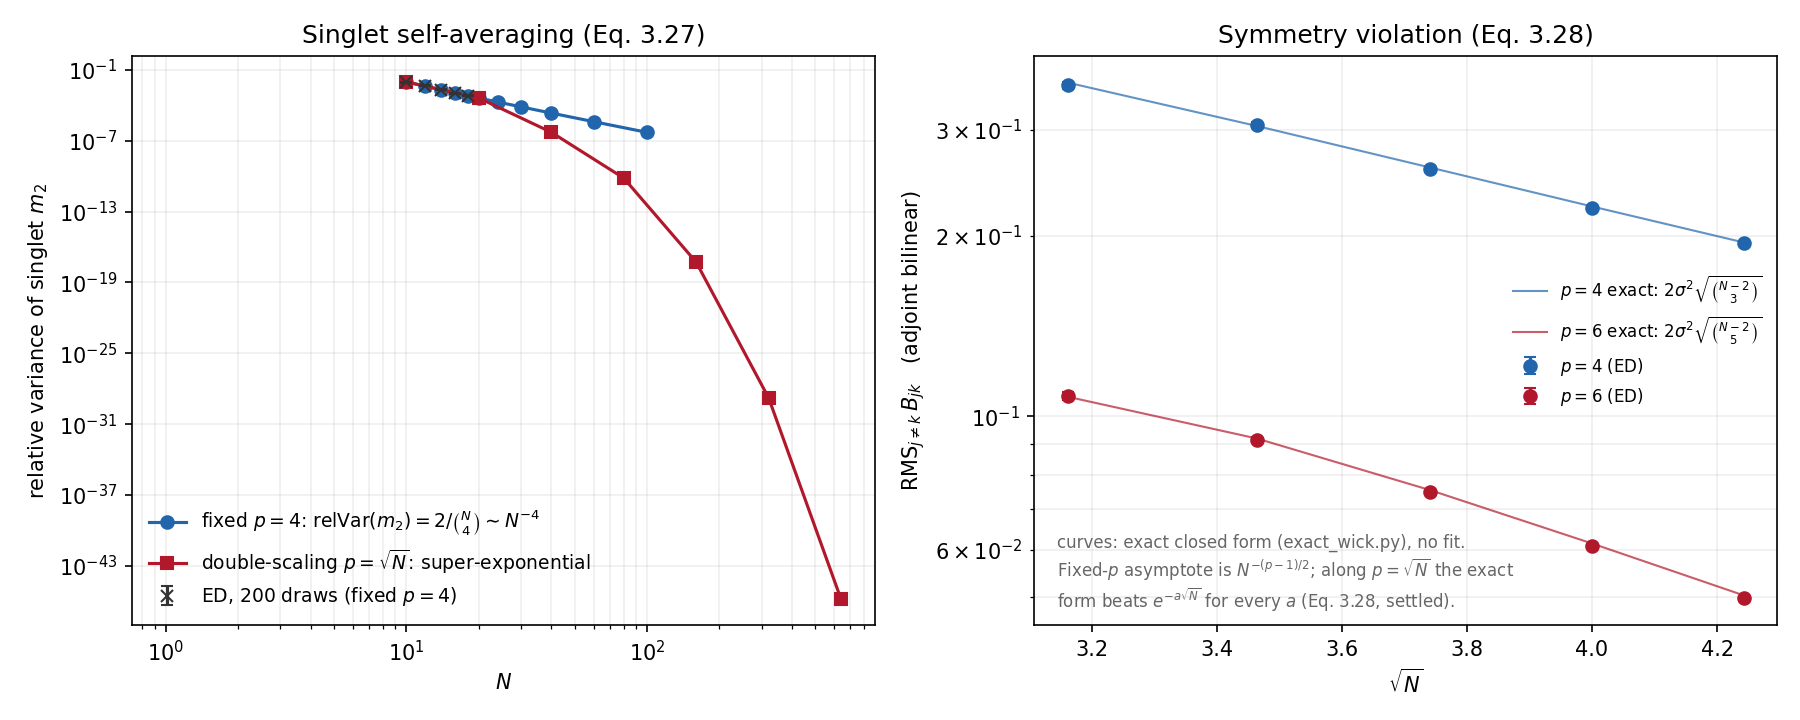
\includegraphics[width=\textwidth]{self_averaging.png}
\caption{Left: the exact singlet rate \eqref{eq:singlet} at fixed $p$
(power law) and along the double-scaling line (super-exponential), with
exact-diagonalization values overlaid. Right: the measured symmetry-violation
signal $\rms_{j\neq k}B_{jk}$ at $p=4,6$ with the exact closed form
\eqref{eq:var} drawn through the points --- no fit.}
\label{fig:main}
\end{figure}

\section{Consequences}

\paragraph{Double scaling: the bound of Eq.~(3.28), exactly.}
Along $p=\sqrt{\lambda N}$, Stirling expansion of Eq.~\eqref{eq:var} gives
\begin{equation}
\ln\rms(B_{jk})\;=\;-\tfrac14\,\sqrt{\lambda N}\,\ln N\,\bigl(1+o(1)\bigr),
\end{equation}
smaller than $e^{-a\sqrt N}$ for \emph{every} $a$: the symmetry-violation
bound of \cite{MSS2607} holds, verified by exact computation in the regime the
bound is about (we have evaluated Eq.~\eqref{eq:var} to $N=1600$, $p=40$),
rather than extrapolated from the $N\le18$ window accessible to exact
diagonalization --- where, we note, fits genuinely cannot discriminate the
competing functional forms.

\paragraph{Fixed $p$: the match regime is only polynomially symmetric.}
The proposed quantitative DSSYK--'t~Hooft comparison --- against the
renormalized-massless meson spectrum of \cite{FLZ} --- must be made at fixed
$p$ and $\lambda\to0$ ('t~Hooft scaling $\bar\alpha=p^2$ fixed)
\cite{MSS2506,MSS2607}. There Eq.~\eqref{eq:var} is the power law
\begin{equation}
\rms(B_{jk})\;\xrightarrow[N\to\infty]{}\;
\frac{2\,p!}{\sqrt{(p-1)!}}\;N^{-(p-1)/2},
\end{equation}
so the emergent gauge symmetry is only polynomially accurate exactly where the
spectra are to be compared --- a quantitative caveat for finite-$N$ tests of
the correspondence. (The pre-asymptotic curvature of Eq.~\eqref{eq:var} over
the ED window closely mimics an exponential; this resolves what the window
fits can and cannot establish.)

\paragraph{The $p=N/2$ artifact, derived.}
Eq.~\eqref{eq:diag} vanishes at $p=N/2$: the ensemble-mean diagonal of the
adjoint bilinear crosses zero there. Ratio diagnostics of the form
$\rms_{\rm off}/\rms_{\rm diag}$ therefore exhibit a spurious spike at
$p\simeq N/2$, which had been observed empirically in exact-diagonalization
studies and is here identified as an exact sign phenomenon
(Lemma~\ref{lem:values}: subsets containing $j$ contribute $-1$).

\section{Corrections to the singlet-tower dictionary}

Setting up the $U(N)$ (Dirac) sector --- complex fermions $c_i$, a
charge-conserving Hamiltonian with $p/2$ creators and $p/2$ annihilators, and
the tower $M_n=\sum_i c_i^\dagger\,(d^n\!/dt^n)c_i$ of \cite{MSS2607},
$\dot X=i[H,X]$ --- yields the following operator facts, each verified to
machine precision and, where stated, forced by symmetry:

\begin{enumerate}
\item $M_0=Q$ exactly (as in \cite{MSS2607}), and $[H,Q]=0$.
\item $M_1=-\tfrac{p}{2}\,iH$, \emph{not} $M_1=H$ as stated in
\cite{MSS2607}: since $\dot Q=0$, $M_1^\dagger=-M_1$ is anti-Hermitian and
cannot equal a nonzero Hermitian operator. Any comparison of ``graviton''
normalizations inherits this factor.
\item Because $M_1$ is conserved,
$0=\dot M_1=\sum_i\bigl(\dot c_i^\dagger\dot c_i+c_i^\dagger\ddot c_i\bigr)$,
hence $M_2=-\sum_i\dot c_i^\dagger\dot c_i$: the identity
$\psi^\dagger\ddot\psi=+\dot\psi^\dagger\dot\psi$ in \cite{MSS2607} has the
wrong sign.
\item $M_n^\dagger=(-1)^nM_n$ holds for $n=0,1,2$ and \emph{fails} for
$n\ge3$: the ordered correlator $\langle M_n(t)M_n^\dagger\rangle$ is then
genuinely asymmetric in frequency, and symmetrized (Hermitian- plus
anti-Hermitian-part) spectral functions are the convention-stable objects.
\item The CP operation assigning $\mathrm{CP}(M_n)=(-1)^{n+1}$ must be the
\emph{unitary} particle--hole map $C$: any antiunitary operation fixing $H$
flips the explicit $i$ in $M_1\propto iH$ and would make the ``graviton''
CP-odd. In the Jordan--Wigner realization
$C=\prod_i(c_i+c_i^\dagger)$ one finds
$Cc_iC^\dagger=(-1)^{N_c-1}c_i^\dagger$ --- a global, mode-independent sign,
invisible to bilinears but essential for odd fermion strings.
\item On $C$-invariant realizations, $\mathrm{CP}(M_0)=-1$ and
$\mathrm{CP}(M_1)=+1$ are exact, but for $n\ge2$ the raw $M_n$ carry
substantial weight in \emph{both} CP channels (up to $\sim\!65\%$ in the
``wrong'' one at accessible sizes): $M_n$ differentiates only one time
argument of the underlying bilinear, and total-time-derivative terms carry the
opposite CP. The assignment $\mathrm{CP}=(-1)^{n+1}$ is therefore a statement
about CP-\emph{resolved} correlators, not about the operators.
\end{enumerate}

\section{Outlook}

The results above settle the self-averaging sector of \cite{MSS2607}
quantitatively: the mechanism is real, its prefactors are now exact, and its
strength in the physically relevant fixed-$p$ regime is known. The open
frontier for the proposed correspondence is the singlet spectrum itself ---
in particular the state/frequency map between the $\omega$-symmetric
infinite-temperature hologram correlators and the KMS-asymmetric Rindler
response of the putative bulk (cf.\ the ``tomperature'' discussion of
\cite{RS}), without which spectral shapes cannot be compared to meson masses
--- and the extraction of the bilinear tower from the exact chord-computed
four-point function of \cite{BINT}.

\paragraph{Acknowledgments.}
% TODO(author): acknowledgments as appropriate.
This note grew out of a computational stress-test of \cite{MSS2607}; all code
and machine-verified derivations are available from the author.

\begin{thebibliography}{9}

\bibitem{MSS2607}
S.~Miyashita, Y.~Sekino and L.~Susskind,
``Holograms and Standard Models,''
arXiv:2607.05678 [hep-th].

\bibitem{SS2501}
Y.~Sekino and L.~Susskind,
``Double-scaled SYK, QCD, and the flat space limit of de Sitter space,''
JHEP \textbf{10} (2025) 137,
arXiv:2501.09423 [hep-th].

\bibitem{MSS2506}
S.~Miyashita, Y.~Sekino and L.~Susskind,
``DSSYK at infinite temperature: the flat-space limit and the 't~Hooft model,''
JHEP \textbf{11} (2025) 107,
arXiv:2506.18054 [hep-th].

\bibitem{FLZ}
V.~A.~Fateev, S.~L.~Lukyanov and A.~B.~Zamolodchikov,
``On mass spectrum in 't~Hooft's 2D model of mesons,''
J. Phys. A \textbf{42} (2009) 304012,
arXiv:0905.2280 [hep-th].

\bibitem{BINT}
M.~Berkooz, M.~Isachenkov, V.~Narovlansky and G.~Torrents,
``Towards a full solution of the large $N$ double-scaled SYK model,''
JHEP \textbf{03} (2019) 079,
arXiv:1811.02584 [hep-th].

\bibitem{GV}
A.~M.~Garc\'ia-Garc\'ia and J.~J.~M.~Verbaarschot,
``Spectral and thermodynamic properties of the Sachdev-Ye-Kitaev model,''
Phys. Rev. D \textbf{94} (2016) 126010,
arXiv:1610.03816 [hep-th].

\bibitem{RS}
A.~Rahman and L.~Susskind,
``Infinite Temperature is Not So Infinite: The Many Temperatures of de Sitter
Space,''
arXiv:2401.08555 [hep-th].

\end{thebibliography}

\end{document}
